\documentclass{article}
\usepackage[margin=1.0in]{geometry}
\usepackage{parskip}
\usepackage{graphicx}
\usepackage{cite}
\usepackage[compact]{titlesec}
\pagestyle{plain}
\topmargin -1.3in
\textheight 9.5in
\oddsidemargin -0.1in
\textwidth 6.8in

\title{\textbf{A Weakly-supervised Approach to Argumentative Zoning of Scientific Documents}}
\author{\normalsize Review by Pranjal Singh(10511)\\}

\titleformat*{\section}{\large\bfseries}
\begin{document}
\maketitle

\section{Overview}
The paper talks about classification of documents according to certain broad classes such as classifying a scientific literature according to objective, methodology, results obtained, etc. using weakly-supervised learning which is less expensive as compared to fully supervised approach. The paper basically investigates the performance of weakly-supervised learning for Argumentative Zoning(AZ) of scientific abstracts. AZ is an approach to information structure which provides an analysis of the rhetorical progression of the scientific argument in a document(Teufel and Moens, 2002). Because of the utility of this method in several domains(such as summarization, computational linguistics), weakly-supervised approach is much more practical.

\section{Architecture}
\textbf{Data:}Guo et al. (2010) provide a corpus of 1000 biomedical abstracts (consisting of 7985 sentences and 225785 words) annotated according to three schemes of information structure. The paper uses AZ (Mizuta et al., 2006)\\ \\
\textbf{Methods:} Comparsion between supervised classifier(SVM and CRF) with four weakly supervised classifiers: two based on semi-supervised learning (transductive SVM and semi-supervised CRF) and two on active learning (Active SVM alone and in combination with self-training).\\
The figure below shows the categories of AZ appearing in the corpus.\\
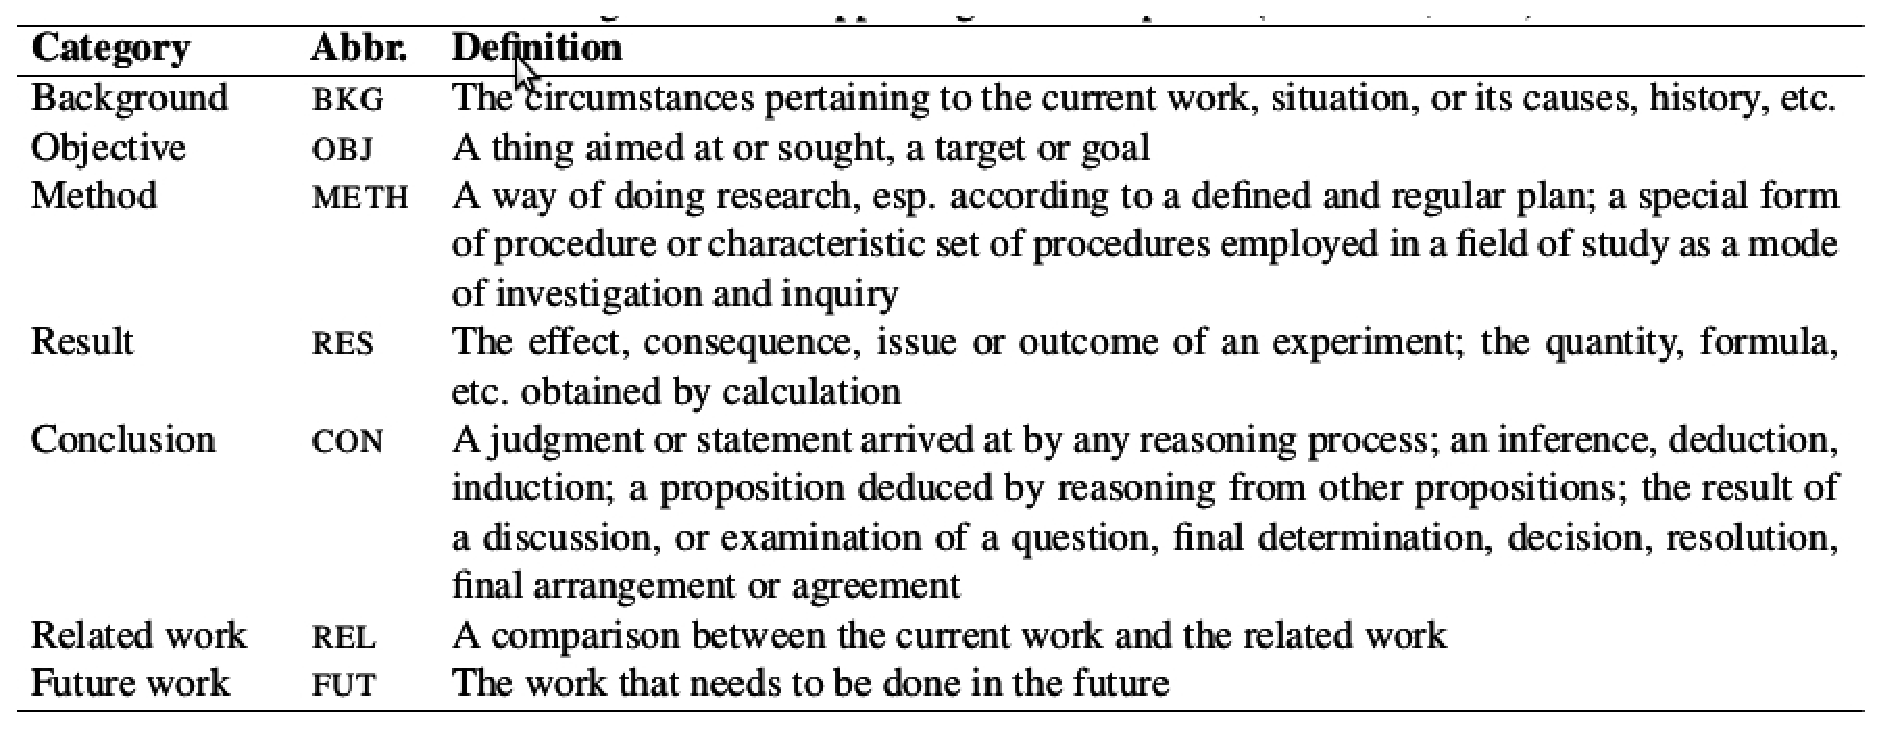
\includegraphics[height=5cm,width=15cm]{1.eps}\\
According to Cohen’s kappa (Cohen, 1960) the inter-annotator agreement is relatively high: kappa(k) = 0.85.

\section{Methodology}
\textbf{Feature Extraction:}Documents were first identified by their features which included Zones(e.g. abstracts were divided into ten parts where zones typically occur), Words, Bi-grams, Verbs, Verb Class, POS, Grammatical Relation, Subject \& Object, Voice of Verbs. These were extracted using tools such as tokenizer(detects boundaries in a sentence), C\&C Tool(POS tagging, lemmatization and parsing), unsupervised spectral clustering method(to acquire verb classes). The lemma output was used to create Word, Bi-gram nad Verb features.\\ \\
\textbf{Machine Learning Methods:} \textbf{SVM} and \textbf{CRF} were used as Supervised methods on the data obtained after feature extraction. \textbf{Active SVM}: \emph{starts with a small amount of labeled data, and iteratively chooses a proportion of unlabeled data for which SVM has less confidence to be labeled and used in the next round of learning}, \textbf{Active SVM with self-training}, \textbf{Transductive SVM}: \emph{takes advantage of both labelled and unlabelled data} and \textbf{Semi-supervised CRF} were used as Weakly-Supervised Methods.

\section{Evaluation}
Results were evaluated in terms of accuracy, precision, recall and F-measure against manual AZ annotation in the corpus. 10-fold cross-validation was used to avoid bias in training data. McNemar's test was used to measure the statistical significance between different ML methods.

\section{Results}
With 10\% training data, ASSVM performs best with 81\% accuracy and macro F-score of .76. ASVM performs with acccuracy of 80\% and F-score of .75. Both of them outperform  supervised SVM. TSVM is the worst performing SVM-based method with an accuracy of 76\% and F-score of .73 which is less than supervised SVM. But it outperforms both CRF-based methods. Only one method(ASVM) identifies six out of the seven possible categories. Other methods identify five categories. RESULTS has the highest amount of data and OBJECTIVE has the minimum. The LOCATION feature is found to be the most important feature for ASSVM. Voice, Verb class and GR contribute to general performance. Least helpful features are Word, Bi-gram and Verb because they suffer from sparse data problems. It was also found that a good performance in fully supervised experiments does not necessarily translate into a good performance in weakly-supervised experiments. The result is attached below:\\
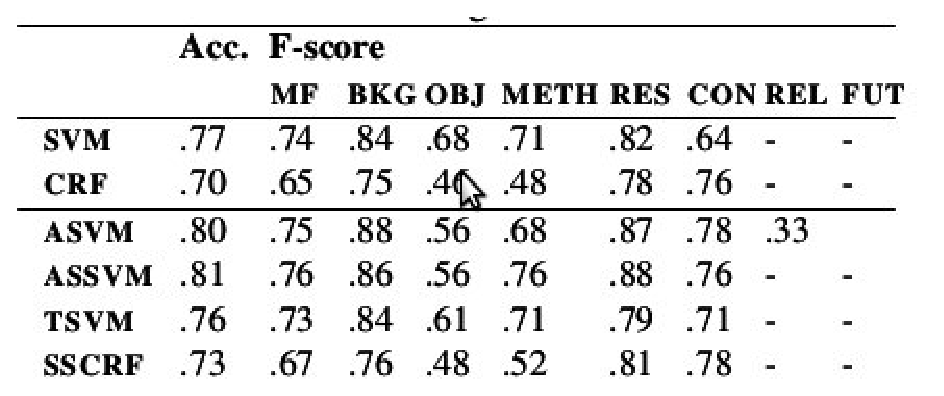
\includegraphics[height=2cm,width=7cm]{2.eps}\\

\section{Discussion}
Almost all the methods performed as they have been performing in other domains and on work done by other authors. BUt TSVM didnot perform better than SVM with the same amount of labelled data. This could be due to higher dimensional data in this work as compared to other works. SSCRF didnot perform as expected on the data may be due to less number of labelled and unlabelled instances.

\section{Future Work}
The approach to active learning could be improved in various ways by experimenting with more complex query strategies such as margin sampling algorithm by (Scheffer et al., 2001) and query-by-committee algorithm by (Seung et al., 1992). Other semi-supervised methods such as Expectation Maximization algorithm could be used which has shown to outperform supervised and transductive SVM. Also, looking for other optimal features could improve the result a lot. It could also be very interesting to evaluate the usefulness of weakly-supervised identification of information structure for NLP tasks such as summarization and information extraction and for practical tasks such as manual review of scientific papers for research purposes.
\nocite{*}
\bibliography{report}{}
\bibliographystyle{plain}
\end{document}
